In this chapter will be described the basic 'How-To' for writing a thesis in \LaTeX

\section{How to cite a reference} 
This is how to cite a reference \cite{Dijkstra68Letters}.

\section{How to include and reference a figure}
As it is possible to see from Figure \ref{fig:sample_figure}, a figure has been included and cited.

\begin{figure}[htbp]
\centering
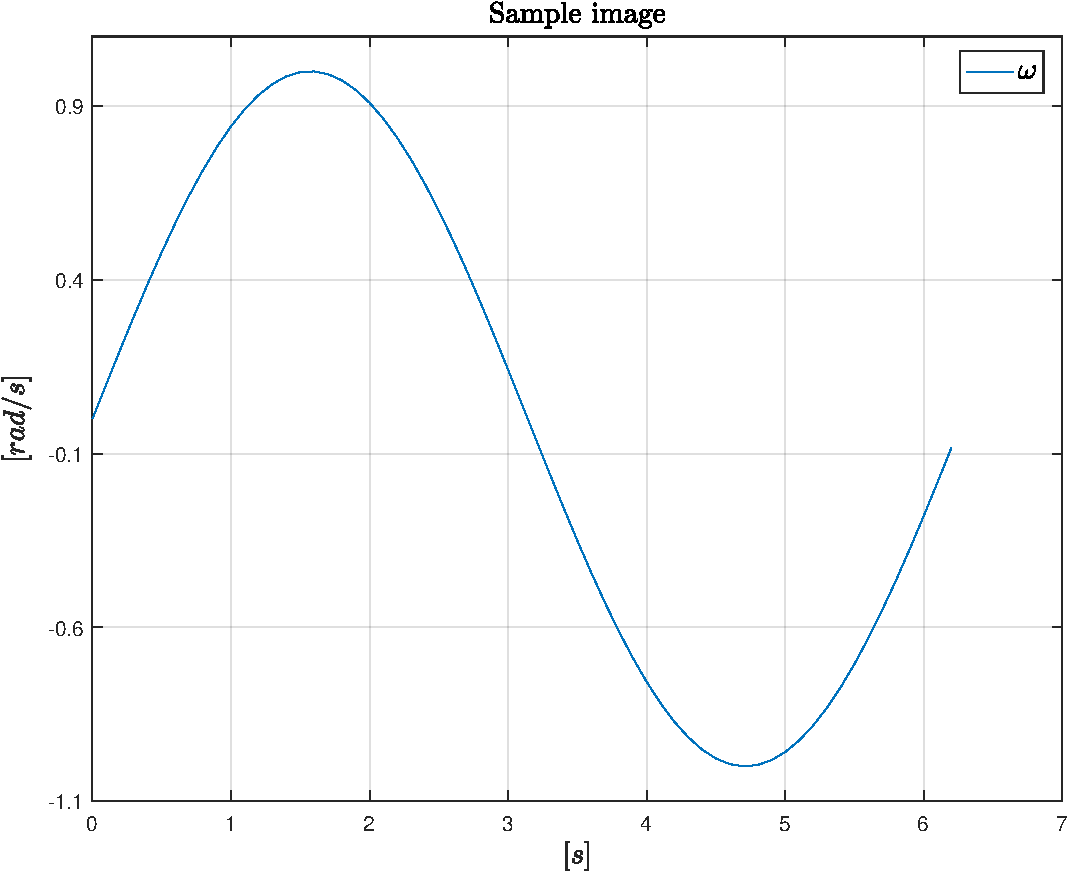
\includegraphics[width = \textwidth]{chapters/chapter-1/figures/sample_figure.pdf}
\caption{Example of a MATLAB plot}
\label{fig:sample_figure}
\end{figure}

\section{How to include and reference an equation}
As it is possible to see from equation \eqref{eq:omega}, an equation has been included and cited.

\begin{equation}
\omega = \sin(t)
\label{eq:omega}
\end{equation}

\section{How to create a table}
Table \ref{tab:sample_table} has been taken as an example from \cite{latexTables}

\begin{table}
\centering
\begin{tabular}{l*{6}{c}r}
Team              & P & W & D & L & F  & A & Pts \\
\hline
Manchester United & 6 & 4 & 0 & 2 & 10 & 5 & 12  \\
Celtic            & 6 & 3 & 0 & 3 &  8 & 9 &  9  \\
Benfica           & 6 & 2 & 1 & 3 &  7 & 8 &  7  \\
FC Copenhagen     & 6 & 2 & 1 & 3 &  5 & 8 &  7  \\
\end{tabular}
\caption{This is a Table}
\label{tab:sample_table}
\end{table}